
\lhead[\chaptername~\thechapter]{\rightmark}


\rhead[\leftmark]{}


\lfoot[\thepage]{}


\cfoot{}


\rfoot[]{\thepage}


\chapter{Systementwicklung}

\section{Anforderungen an das System}

	\subsection{N"otige Aufl"osung}
	
		\subsubsection*{Frequenz}
		
		\subsubsection*{Ausdehnung}

	\subsection{Gr"o"se}
	
	\subsection{Position am Brustkorb}
	
		\subsubsection*{Unter Belastungsbedingungen}
		Brustatmung
		
		\subsubsection*{In Ruhe}
		Bauchatmung
	
	\subsection{Rotations- und Translationsbewegungen}
	
\section{Verwendete ICs}

	\subsection{STM32F405RG}
	
	\subsection{MPU9250}
	
	\subsection{(Bluetooth-Modul)}
	
\section{Platinendesign}

\newpage

\section{Kalibrierung}

	\begin{figure}[h]
		\centering
		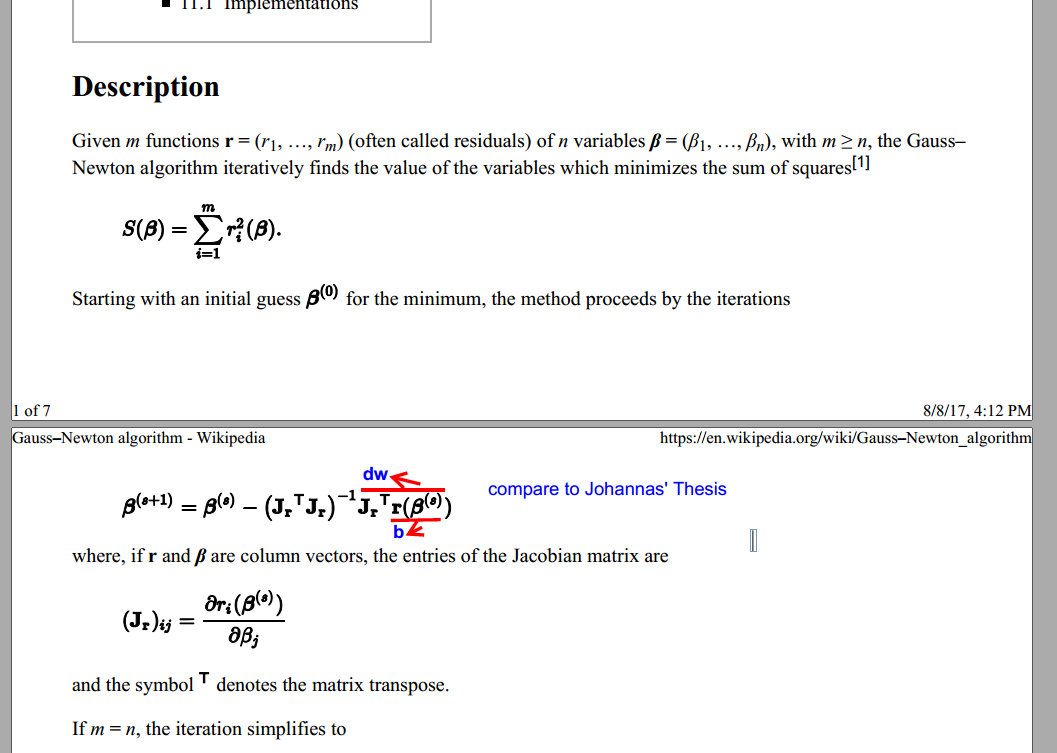
\includegraphics[width=1\textwidth]{images/kalibrierung_algo}
		\caption[Flow-Chart des Kalibrierungsalorithmus]{Der Kalibrierungsalorithmus berechnet den Offset der Drehratenratensensoren und die Erdbschleunigung der Beschleunigungssensoren in Ruhe. Nach Berechnung der Roll- und Nickwinkel wird der Gierwinkel mit der kleinsten Abweichung mittels sukzessiver Approximation in vier Schritten bestimmt. Zuletzt wird die Rotationsmatrix übergeben und die zukünftigen Messdaten mit ihr rotiert.}
		\label{img:kalibrierung-algo}
	\end{figure}

	\begin{figure}[h]
		\centering
		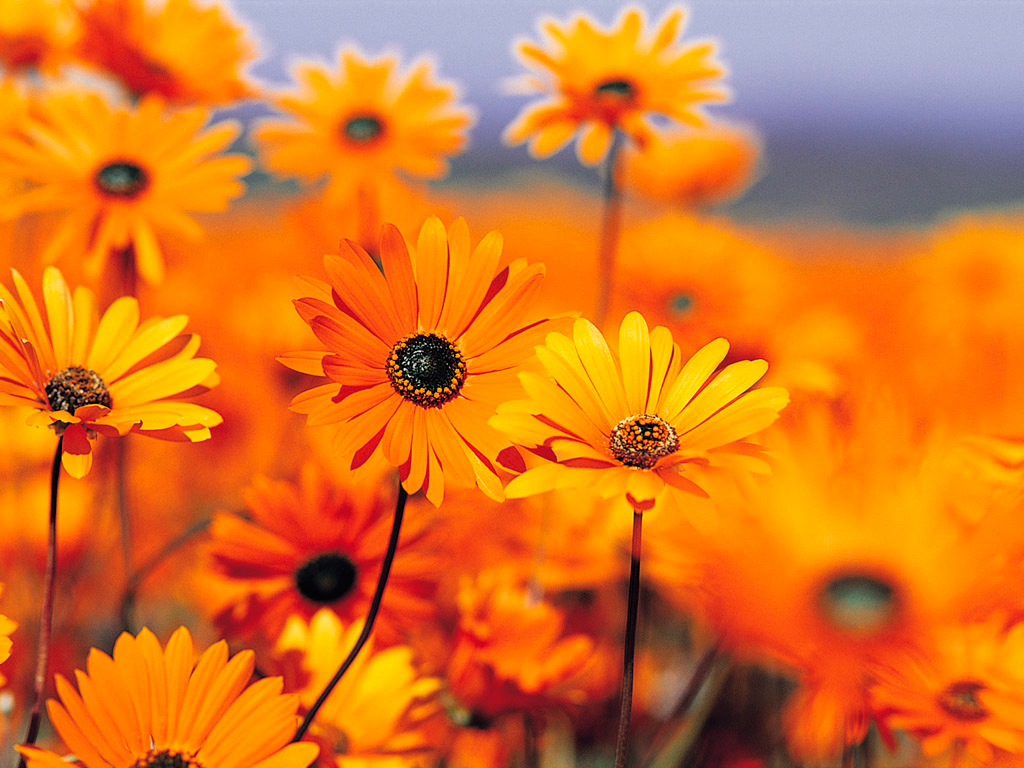
\includegraphics[width=1\textwidth]{images/Messergebnisse/calibration-sar-error}
		\caption[Abweichung der Voder- und Rückvektoren]{.}
		\label{img:kalibrierung-sar-error}
	\end{figure}

	\begin{figure}[h]
		\centering
		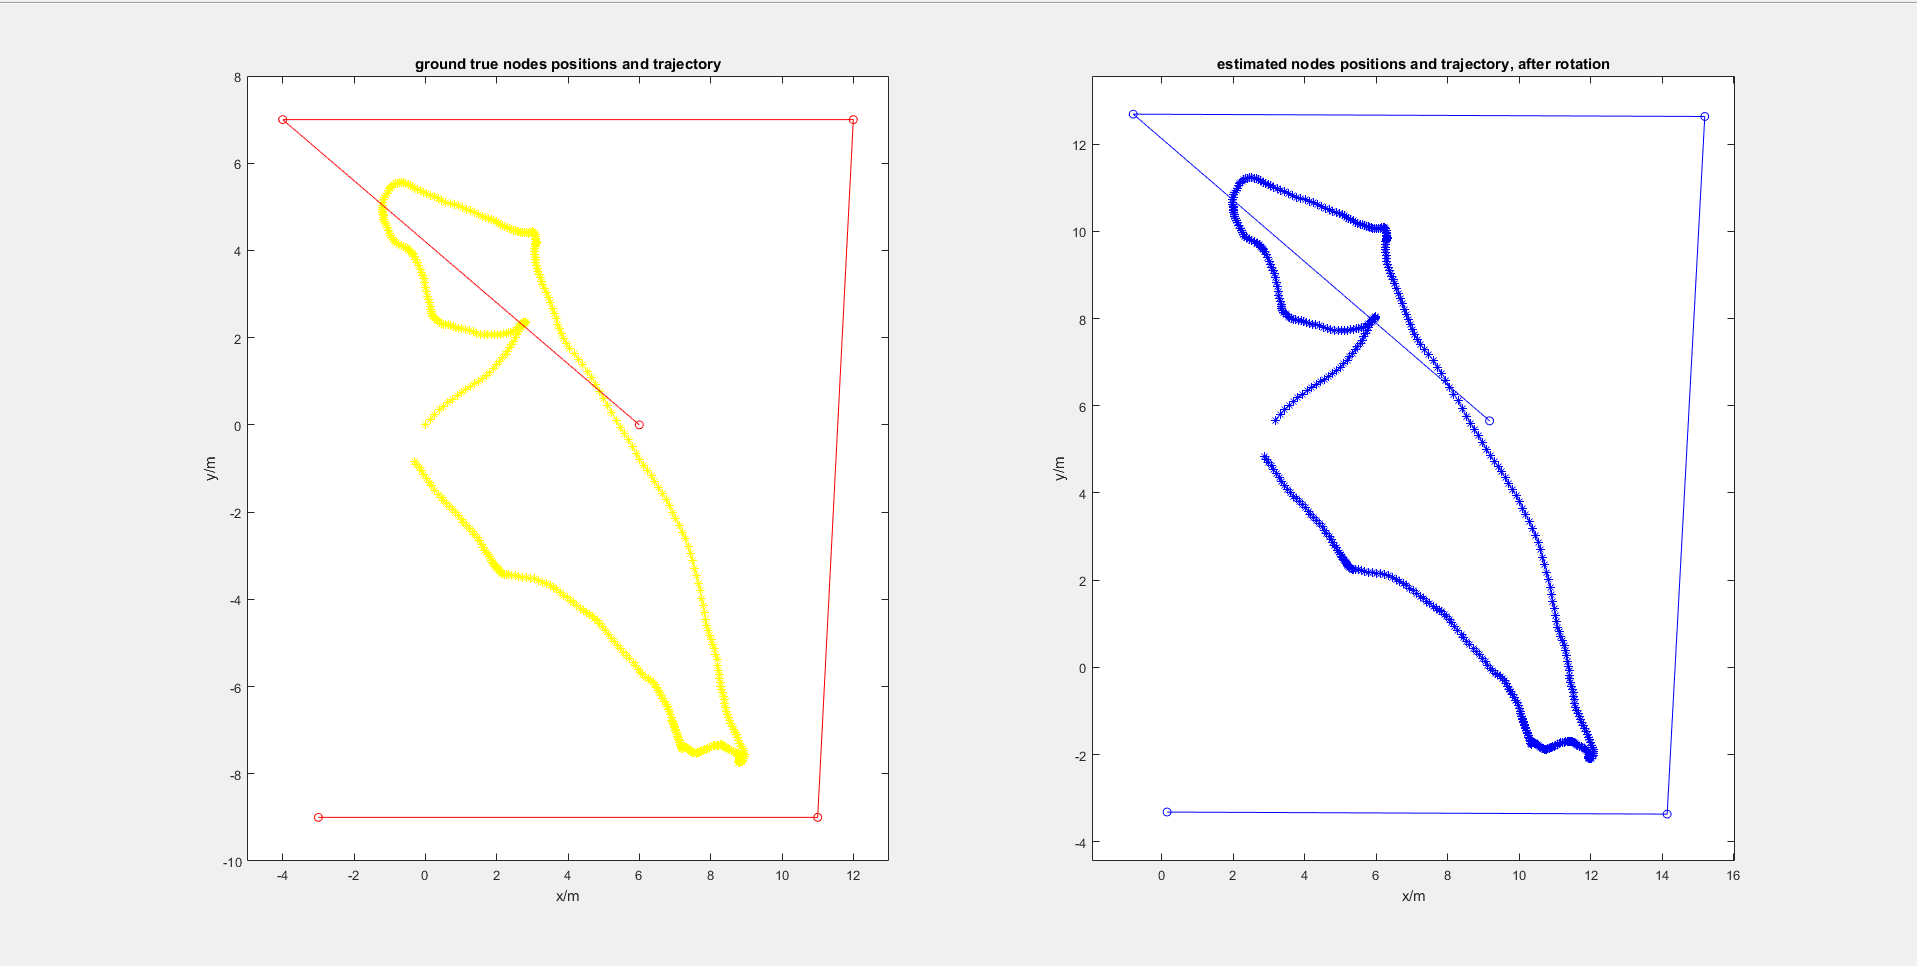
\includegraphics[width=1\textwidth]{images/kalibrierung_sar}
		\caption[Sukzessive Approximation]{Das Verfahren der sukzessiven Approximation wird verwendet, um den Gierwinkel zwischen den Vorder- und Hinterachsen zu bestimmen. Dabei wird bei jedem Schritt die Abweichung zueinander nach Rotation um den Gierwinkel berechnet und der Gierwinkel dann schrittweise approximiert.}
		\label{img:sar}
	\end{figure}


	\begin{table}[h!]
		\centering
		\caption{Arbeitsweise der Sukzessiven Approximation}
		\label{tab:sar}
		\begin{tabular}{ccccc}
			\toprule
			Schritt & \multicolumn{2}{c}{Abweichungen} & Addierter Winkel & Gesamtwinkel\\
			& Untereinander & Zum vorherigen & in $^\circ$& in $^\circ$\\
			\midrule
			1 & E$_{1,p}$ < E$_{1,n}$ 	& -	& +8  & 8 \\
			2 & E$_{2,p}$ < E$_{2,n}$ 	& E$_{2,p}$ < E$_{1,p}$	& +4 & 12\\
			3 & E$_{3,p}$ > E$_{3,n}$ 	& E$_{3,n}$ < E$_{2,p}$	& $-$2  & 10 \\
			4 & E$_{4,p}$ < E$_{4,n}$ 	& E$_{4,p}$ > E$_{3,n}$	& +0  & 10 \\
			5 & E$_{5,p}$ < E$_{5,n}$ 	& E$_{5,p}$ > E$_{3,n}$	& +0  & 10 \\
			6 & E$_{6,p}$ < E$_{6,n}$ 	& E$_{6,p}$ < E$_{3,n}$	& +0,25  & 10,25 \\
			\bottomrule
		\end{tabular}
	\end{table}